\chapter{Эксперимент 4}

\begin{enumerate}
	\item Настроил осциллограф на измерение временной развертки сигнала
	генератора: частота генератора $1$кГц, амплитуда $10$В.
	\begin{figure}[H]
		\centering
		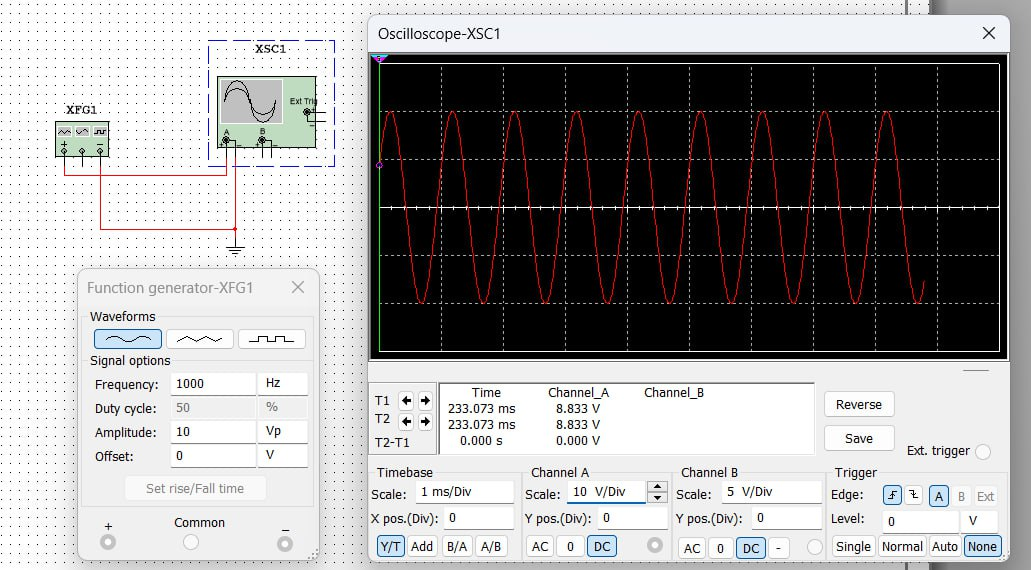
\includegraphics[width=0.6\textwidth]{img/24.jpg}
	\end{figure}
	
	\item Собрал схему со своим диодом
	\begin{figure}[H]
		\centering
		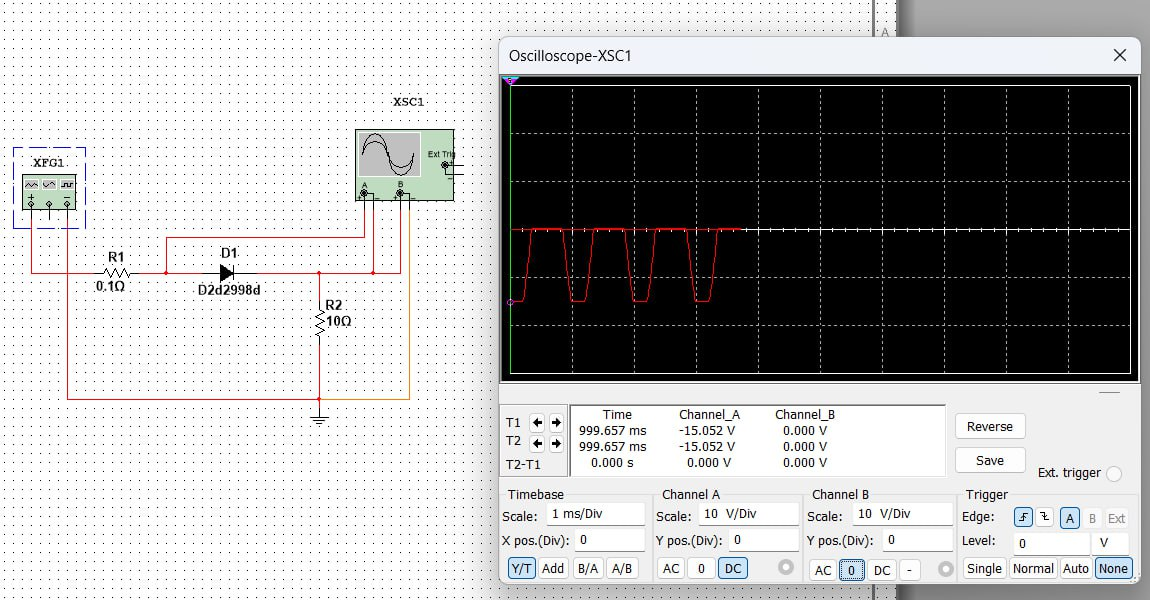
\includegraphics[width=0.6\textwidth]{img/25.jpg}
	\end{figure}
	
	\begin{figure}[H]
		\centering
		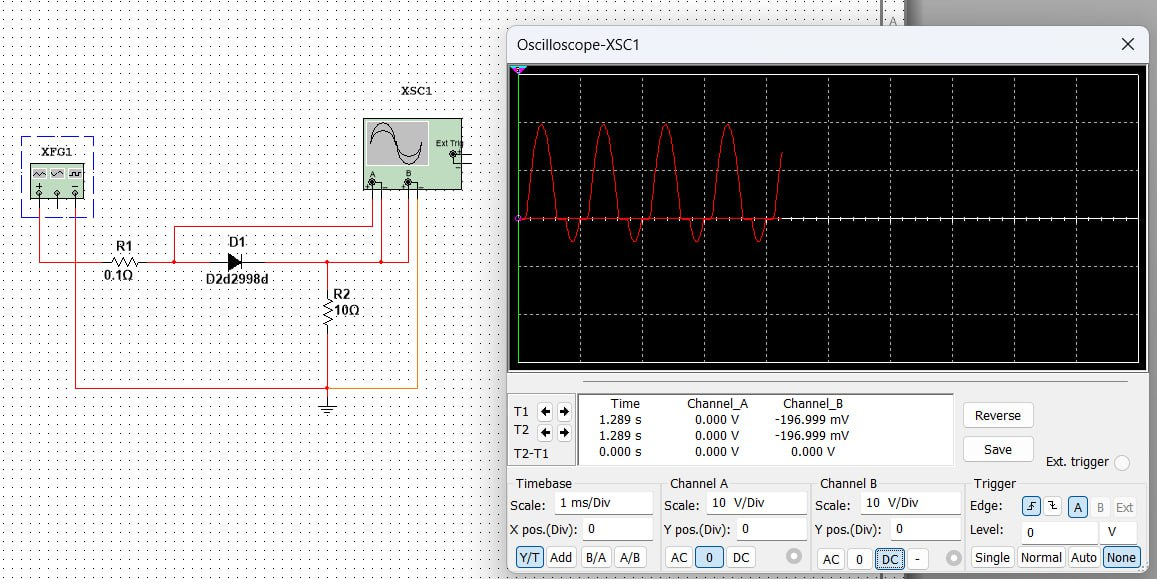
\includegraphics[width=0.6\textwidth]{img/26.jpg}
	\end{figure}
	\newpage
	\item Параллельно нагрузочному резистору поставил накопительный конденсатор,
	среднее напряжение выросло. Получился однополупериодный выпрямитель.
	\begin{figure}[H]
		\centering
		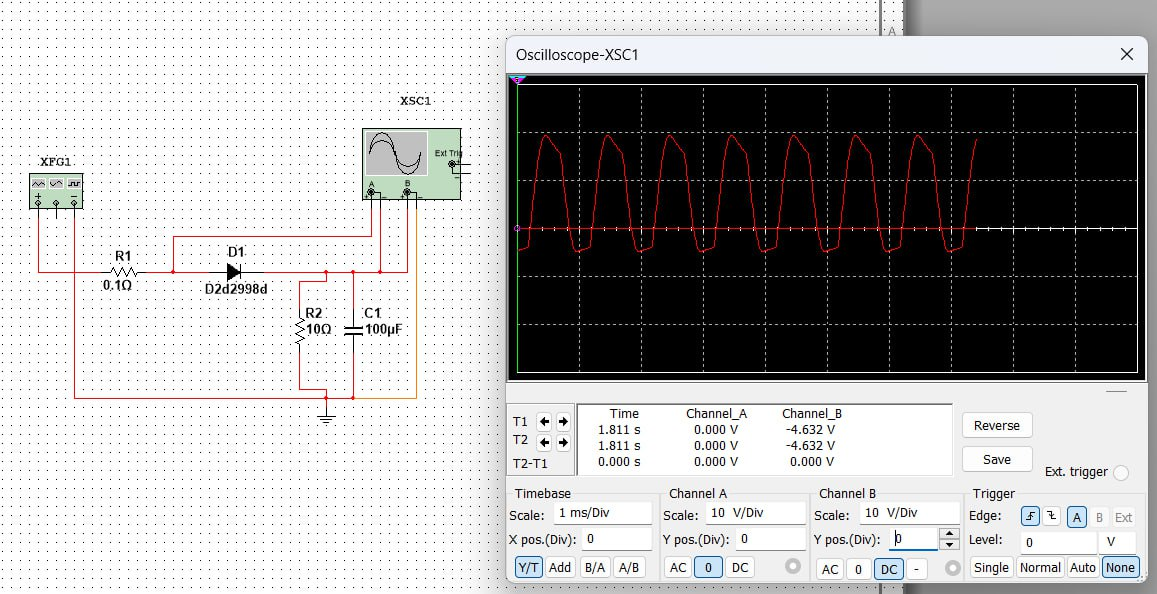
\includegraphics[width=0.6\textwidth]{img/27.jpg}
	\end{figure}
\end{enumerate}
